\documentclass[]{article}

% Packages
%\usepackage[dvipsnames]{xcolor}  % for coloring
\usepackage{titling}	% for subtitle custom command

%for flowchart:
\usepackage{amsmath}
\usepackage{amssymb}
\usepackage{graphicx}
\usepackage{siunitx}
\usepackage[a4paper,left=3cm,right=2cm,top=2.5cm,bottom=2.5cm]{geometry}
\usepackage{tikz}
\usetikzlibrary{patterns}
\usepackage{caption}
\usetikzlibrary{arrows}
\usepackage{color}
\usepackage[colorlinks]{hyperref}
\usepackage{pgfplots}
\usepackage{listings}
\usepackage[utf8]{inputenc}
\usetikzlibrary{shapes.geometric}
\usepackage{tikz-cd}
\usetikzlibrary{positioning}
\tikzset{
	shift left/.style ={commutative diagrams/shift left={#1}},
	shift right/.style={commutative diagrams/shift right={#1}}
}


% for code snippets
\usepackage{listings}
\usepackage{color}
\definecolor{dkgreen}{rgb}{0,0.6,0}
\definecolor{gray}{rgb}{0.5,0.5,0.5}
\definecolor{mauve}{rgb}{0.58,0,0.82}
\lstset{frame=none,
	language=Java,
	aboveskip=3mm,
	belowskip=3mm,
	showstringspaces=false,
	columns=flexible,
	basicstyle={\small\ttfamily},
	numbers=none,
	numberstyle=\tiny\color{gray},
	keywordstyle=\color{blue},
	commentstyle=\color{dkgreen},
	stringstyle=\color{mauve},
	breaklines=true,
	breakatwhitespace=true,
	tabsize=3
}


% Algorithms
\usepackage{algorithm}
\usepackage{algorithmicx}
\usepackage[noend]{algpseudocode}
\newcommand{\Get}{\State \textbf{get}~}
\newcommand{\Set}{\State \textbf{set}~}
\newcommand{\Print}{\State \textbf{print}~}
\newcommand{\Getx}[1]{\Statex \algindent{#1} \textbf{get}~}		% x denotes non-numbered lines
\newcommand{\Setx}[1]{\Statex \algindent{#1} \textbf{set}~}	% enter the number of lines to indent
\newcommand{\Printx}[1]{\Statex \algindent{#1} \textbf{print}~}
\newcommand{\Stop}{\State \textbf{stop}~}
\newcommand{\algindent}[1]{\Repeat{#1}{\hskip\algorithmicindent}}
\algdef{SE}[DOWHILE]{Do}{doWhile}{\algorithmicdo}[1]{\algorithmicwhile\ (#1)}

%tables for list representation
\usepackage{arydshln, collcell}
\newcolumntype{C}{>{\collectcell\mathsf}c<{\endcollectcell}}


% Fixes weird backwards quote thing
\usepackage [english]{babel}
\usepackage [autostyle, english = american]{csquotes}
\MakeOuterQuote{"}

% fix upside down exclaimation points for less thans or greater thans
\usepackage[T1]{fontenc}

% stop indentation
\setlength{\parindent}{0pt}


% Custom Commands
\newcommand{\subtitle}[1]{
	\posttitle{
		\par\end{center}
	\begin{center}\large#1\end{center}
	\vskip0.5em}
}


% My colors
\colorlet{mygray}{gray!3}
\colorlet{myyellow}{yellow!40}
\colorlet{mygreen}{green!40}
\colorlet{myblack}{black!40}
\colorlet{myblue}{blue!28}


% Title
\title{\textbf{CS 211 Notes}}
\subtitle{Introduction to Programming}
\author{Jaeden Bardati}
\date{\textit{Last modified \today}}

\setcounter{section}{-1}	% 0-indexes the section

\begin{document}

\maketitle
\bigbreak

% Course Video 1
\section{Course Overview\\ {\large \normalfont September 10, 2021}}
\bigbreak

\subsection{Objectives}
\bigbreak

The course is intended to teach how to develop a computer program to solve a problem. C++ is a tools that will be used to develop these skills and logical thinking. These skills will be transferable to other languages.

\section{Computer Organization}
\bigbreak

% Course Video 2
\subsection{Hardware\\ {\large \normalfont September 11, 2021}}
\bigbreak

\subsubsection{Components}
\bigbreak

Modern computers are built using the \textbf{Von Neumann machine}. There are three aspects:

\begin{itemize}
	\item \textbf{Architecture}: \textbf{I/O} (User interaction) + \textbf{Memory} (Storage) + \textbf{CPU} (\textit{CU}: Control Unit, \textit{ALU}: Arithmetic and Logic Unit). These are all connected by a shared bus.
	\item \textbf{Stored Programs}: All programs and data are stored in memory (binary).
	\item \textbf{Sequential Execution}: Also called the \textbf{fetch-decode-execute} cycle. Instructions are \textbf{fetched} from memory, \textbf{decoded} by the CU and then \textbf{executed} by the ALU. If there is a result, it is stored back in memory. \smallskip
\end{itemize}

% Course Video 3
\subsection{Memory\\ {\large \normalfont September 11, 2021}}
\bigbreak

The memory is organized in a \textbf{hierarchy}. At the bottom of the hierarchy is the Hard Drive (in TB). At the top is the CPU. Since the hard drive is slow, when some data from the hard drive is needed, it is first loaded into \textbf{RAM (Random Access Memory)} (in GB). The RAM is still too slow for the RAM, so the data is stored in \textbf{cache} (in KB or MB). Yet still, this is not fast enough for the CPU, so \textbf{registers} (in Bytes) in the CPU itself are used to store variables.

\begin{center}
	\tikzstyle{top} = [rectangle, minimum width=3cm, minimum height=1cm, text centered, draw=black, fill=purple!30]
	\tikzstyle{medtop} = [rectangle, minimum width=5cm, minimum height=1cm, text centered, draw=black, fill=red!30]
	\tikzstyle{medbot} = [rectangle, minimum width=8cm, minimum height=1cm, text centered, draw=black, fill=orange!30]
	\tikzstyle{bot} = [rectangle, minimum width=12cm, minimum height=1cm, text centered, draw=black, fill=yellow!30]
	
	\begin{tikzpicture}[node distance=2cm, >=latex', auto, thick]
		\node (ntop) [top] {CPU};
		\node (nmedtop) [medtop, below of=ntop] {Cache};
		\node (nmedbot) [medbot, below of=nmedtop] {RAM (Random Access Memory)};
		\node (nbot) [bot, below of=nmedbot] {Hard Drive};
		
		\path[->, shift left=2em]
			(ntop) edge node {store} (nmedtop)
			(nmedtop) edge node {load} (ntop);
		\path[->, shift left=3.5em]
			(nmedtop) edge node {update} (nmedbot)
			(nmedbot) edge node {load} (nmedtop);
		\path[->, shift left=6em]
			(nmedbot) edge node {save} (nbot)
			(nbot) edge node {load} (nmedbot);	
	\end{tikzpicture}
\end{center}
\bigbreak

\noindent As you \textbf{go up} the hierarchy, the \textbf{speed increases}, but the \textbf{size decreases} and the \textbf{cost increases}.

\subsubsection{RAM}
\bigbreak

Random access memory is organized in an array of Bytes ("words"). \\\\
Words in RAM are addressed with a byte themselves (e.g. 01101101 is an address). These are typically written in hexadecimal (e.g. 6D). \\\\
Words in RAM can be data or machine code instructions. Instructions contain a binary code for each operation (for example, addition). Instructions codes are dependent on the CPU.


\section{C++ Programming}
\bigbreak

% Course Video 7
\subsection{A Flow Chart: Program to Binary\\ {\large \normalfont September 12, 2021}}
\bigbreak

This is a flow chart of what is done by the computer when compiling a C++ file. In blue is the Python equivalent.

\begin{center}
	\tikzstyle{greenbox} = [rectangle, minimum width=3cm, minimum height=1cm, text centered, draw=black, fill=green!30]
	\tikzstyle{bluebox} = [rectangle, minimum width=3cm, minimum height=1cm, text centered, draw=black, fill=blue!30]
	\tikzstyle{arrow} = [thick,->,>=stealth]
	
	\begin{tikzpicture}[node distance=2cm, >=latex', auto, thick]
		\node (editfile) [greenbox] {Edit file.cpp};
		\node (compile) [greenbox, below of=editfile] {Compile};
		\node (instructions) [greenbox, below of=compile] {Machine Code instructions};
		\node (libraries) [greenbox, left of=compile, xshift=-2cm] {Libraries};
		\node (linker) [greenbox, below of=instructions] {Linker};
		\node (executable) [greenbox, below of=linker] {Executable};
		\node (python) [bluebox, right of=editfile, xshift=2cm] {Python};
		\node (compile2) [bluebox, right of=compile, xshift=2cm] {Compile};
		
		\draw [arrow] (editfile) -- (compile);
		\draw [arrow] (compile) -- (instructions);
		\draw [arrow] (instructions) -- (linker);
		\draw [arrow] (linker) -- (executable);
		\draw [arrow] (libraries) |- (linker);
		\draw [arrow] (python) -- (compile2);
		\draw [arrow] (compile2) |- (instructions);
		\draw [arrow] (compile2) |- (executable);
	\end{tikzpicture}
\end{center}
\bigbreak

\noindent Note that the bottom of the flow chart is the same for all programming languages, because in all languages, CPU-specific machine code is needed to execute code.\\

\noindent The process of catching errors is as according to the following flow chart.

\begin{center}
	\tikzstyle{yellowbox} = [rectangle, minimum width=3cm, minimum height=1cm, text centered, draw=black, fill=yellow!30]
	\tikzstyle{reddiamond} = [diamond, minimum width=2cm, minimum height=2cm, text centered, draw=black, fill=red!30]
	\tikzstyle{arrow} = [thick,->,>=stealth]
	
	\begin{tikzpicture}[node distance=2cm, >=latex', auto, thick]
		\node (edit) [yellowbox] {Edit};
		\node (compile) [yellowbox, below of=edit] {Compile};
		\node (error) [reddiamond, below of=compile, yshift=-0.4cm] {Error};
		\node (test) [yellowbox, below of=error, yshift=-0.4cm] {Test};
		\node (runtimeerror) [reddiamond, below of=test, yshift=-0.8cm] {Runtime Error};
		\node (useit) [yellowbox, below of=runtimeerror, yshift=-0.8cm] {Use it};
		
		\draw [arrow] (edit) -- (compile);
		\draw [arrow] (compile) -- (error);
		\draw [arrow] (error) -- node[anchor=west] {no} (test);
		\draw [arrow] (test) -- (runtimeerror);
		\draw [arrow] (runtimeerror) -- node[anchor=east] {no} (useit);
		\draw [arrow] (error) -- node[anchor=north, yshift=-0.1cm] {yes} ++(-2.5cm,0) |- (edit);
		\draw [arrow] (runtimeerror) -- node[anchor=north, yshift=-0.1cm] {yes} ++(2.5cm,0) |- (edit);
	\end{tikzpicture}
\end{center}
\bigbreak

\noindent In this context, \textbf{errors} are caught by the compiler. This is opposed to \textbf{runtime errors}, which are not caught by the compiler. These can be something like division by zero or infinite loops.

% Course Video 4, 5, 6 for code blocks setup and first code.
\subsection{First C++ Code\\ {\large \normalfont September 12, 2021}}
\bigbreak

The following code is a hello world program in C++.

\begin{lstlisting}
	// helloworld.cpp
	#include <iostream>		// include statement allows the use of C++ libraries
	#include <stdio.h>		// this library contains getchar()
	
	using namespace std;	// a standard environment (input from keyboard, output is the screen)
	
	int main() {
		
		cout << "Hello world!" << endl;		// Prints "Hello world!" to the screen
		
		getchar();      // wait for user to type a character
		
		return 0;		// 0 means that the execution was successful
	}
\end{lstlisting}
\bigbreak

\subsection{Data types\\ {\large \normalfont September 12, 2021}}
\bigbreak

Variables are referred to as identifiers. Identifiers are memory locations accessed and modified. \\\\
Inside a main function (as above), the following code declares a variable of integer type in C++. 

\begin{lstlisting}
	int numYears;       // allocated space in memory to contain num of years
\end{lstlisting}
\bigbreak

You can also initialize the variable with a value on declaration:
\begin{lstlisting}	
	int number = 5;     // declare and initialize (give a value too)
\end{lstlisting}
\bigbreak

Some rules to follow when naming variables are:
\begin{itemize}
	\item Names have meanings
	\item Must be case sensitive (e.g. numYears is not numyears)
	\item Consists of letters, numbers and underscores
	\item First character cannot be a number
\end{itemize}
\bigbreak

Some types of variables are:
\begin{itemize}
	\item Integers (e.g. -5, 0, +2) [int]
	\item Real numbers (floating point numbers or doubles, e.g. 2.453, -4.1987e7) [float or double]
	\item Booleans (e.g. true, false) [bool]
	\item Characters [char]
\end{itemize}	    
\bigbreak

You can assign a value to a variable after declaring it:
\begin{lstlisting}	
	int width, height;
	int area;
	
	width = 5;
	height = 3;
	
	area = width * height;
\end{lstlisting}
\bigbreak

Constants (denoted with the keyword "const") cannot be changed throughout the program. The convention is to use capital letters for constants.
\begin{lstlisting}	
	const double PI = 3.14159265;

	int radius = 6;
	double area = PI * radius * radius;
\end{lstlisting}
\bigbreak

You would get an error if you were to try to reassign a constant.
\begin{lstlisting}
	const double PI = 3.14159265;
	PI = 3.14; 	/// ERROR
\end{lstlisting}
\bigbreak

\subsection{Arithmetic operations\\ {\large \normalfont September 22, 2021}}
\bigbreak

There are 5 basic arithmetic operations supported by C++
\begin{itemize}
	\item Addition (+)
	\item Subtraction (-)
	\item Multiplication (*)
	\item Division (/)
	\item Modulus or "Remainder" (\%)
\end{itemize}
\bigbreak

For example,

\begin{lstlisting}
	int a = 5;
	int b = 2;
	
	cout << a + b / 2 << endl;			/// 6
	cout << (a + b) / 2 << endl;		/// 3
	cout << a / 2 + 3 << endl;			/// 5
	cout << a / b / 3 << endl;			/// 0
\end{lstlisting}
\bigbreak

This is done with integer operations since both arguments of each operation are integers (round down if the result of a division is a decimal). If one argument is a double/float, the result is a double/float. For example,

\begin{lstlisting}
	int a = 5;
	int b = 2;
	
	cout << a + b / 2 << endl;			/// 6
	cout << (a + b) / 2 << endl;		/// 3.5
	cout << a / 2 + 3 << endl;			/// 5
	cout << a / b / 3 << endl;			/// 0.83333333
\end{lstlisting}

\subsubsection{Assigning and operations}

When you are assigning a variable and performing an operation to it at the same time you can do the following:

\begin{lstlisting}
	int x = 25;
	
	x += 1		// equivalent to x = x + 1  (or x++)
	x -= 2;		// equivalent to x = x - 2
	x *= 3;		// equivalent to x = x * 3
	x /= 4;		// equivalent to x = x / 4
	x %= 5;		// equivalent to x = x / 5
\end{lstlisting}


\subsubsection{Division when initializing or assigning a variable}

Naively, to initialize a variable to the result of a division, you could try

\begin{lstlisting}
	int div = 7/3;		/// 2
\end{lstlisting}
\bigbreak

However, this results in 2, not the desired result of 2.3333. You could also try changing the variable type

\begin{lstlisting}
	double div = 7/3;		/// 2
\end{lstlisting}
\bigbreak

This does not work either, since the integer division happens before the result is assigned to the variable div. Instead, you have to force the compiler to recognize an argument as a float.

\begin{lstlisting}
	double div = 7.0/3;		/// 2.333333
\end{lstlisting}
\bigbreak

If instead you had decided to make the variable type of div and integer and run it

\begin{lstlisting}
	int div = 7.0/3;		/// 2
\end{lstlisting}
\bigbreak

It will perform the double operation, but save it in var as an integer. \\\\

A way of doing the float operation with two integers is by \textbf{casting} types. This can be done as follows.

\begin{lstlisting}
	double div = (double) 7/3;		/// 2.333333
	double div2 = 7/(double)3;		/// 2.333333
	
	int c = 7
	double div3 = (double) c/3;		/// 2.333333
	// Note, this does not change the type of c.
\end{lstlisting}
\bigbreak

The remainder (\%) operation returns the remainder of the division between two integers:

\begin{lstlisting}
	cout << 7 % 3 << endl;		/// 1
	cout << 10 % 6 << endl;		/// 4
	cout << 13 % 4 << endl;		/// 1
\end{lstlisting}

\subsubsection{Type conversion}

We can also convert types from doubles to integers by truncation or rounding: 

\begin{lstlisting}
	double price = 2.55;
	
	int sum = price;		/// truncate
	int sum2 = price + 0.5 	/// round to the nearest int
\end{lstlisting}


\subsection{I/Os\\ {\large \normalfont September 22, 2021}}
\bigbreak


To do this, we will use the iostream library and standard namespace.

\begin{lstlisting}
	#include <iostream>
	using namespace std;
\end{lstlisting}

\subsubsection{Reading inputs}

You can get input from the keyboard using cin. For example,

\begin{lstlisting}
	int number;
	
	cout << "Please enter a value between 0 and 10." << endl;
	
	cin >> number;		// reads integer
	
	cout << "The entered number is " << number;
\end{lstlisting}
\bigbreak

You can also get multiple variables with the same cin.

\begin{lstlisting}
	int length, width;
	
	cout << "Please enter the length and width of the rectangle: ";
	
	cin >> length >> width;
	
	int area = length * width;
	cout << "The area is " << area
\end{lstlisting}
\bigbreak

\subsubsection{Formatting outputs}

When outputting the result of a float, we inevitably run into an issue:

\begin{lstlisting}
	double result = 123456789.1284567;		/// 1.23457e+008
	
	cout << result << endl;
\end{lstlisting}
\bigbreak

This returns 1.23457e+008. To see all the digits, we must first pass result to fixed before cout.
\begin{lstlisting}
	double result = 123456789.1284567;
	
	cout << fixed << result << endl;		/// 123456789.128457
\end{lstlisting}
\bigbreak

To properly format the output of doubles, we must include the iomanip library and use the setprecision(n) function.

\begin{lstlisting}
	#include <iomanip>
	
	double result = 123456789.1284567;
	
	cout << fixed << setprecision(2) << result << endl;		/// 123456789.13
	cout << result << endl;									/// 123456789.13
\end{lstlisting}
\bigbreak

This rounds the double to the nearest nth decimal. Note that result will now format that way if outputted without the fixed and setprecision call. However, this does not actually change the value of the result variable. 

\begin{lstlisting}
	double result2 = result + 1;
	
	cout << setprecision(3) << result2 << endl;			/// 123456790.128
\end{lstlisting}
\bigbreak

Finally, to set a limit to the number of characters that are displayed to an integer n, we can use the setw(n) function from the iomanip library like this

\begin{lstlisting}
	cout << fixed << setprecision(2) << setw(15) << left << result << "End of line" << endl;
\end{lstlisting}
\bigbreak

The result is "123456789.13~~~End of line". Note the exactly 15 characters until "End of line".

\subsection{Strings\\ {\large \normalfont September 22, 2021}}
\bigbreak

To use strings, you have to include the string library:

\begin{lstlisting}
	#include <string>
\end{lstlisting}

\subsubsection{Declaration}

You can declare, initialize, assign, and output strings as such
\begin{lstlisting}
	string lname;
	string fname = "Jaeden";
	lname = "Bardati";
	
	cout << fname << " " << lname;		/// Jaeden Bardati
\end{lstlisting}

\subsubsection{Concatenation}

To combine strings together, we must use \textbf{concatenation}.
\begin{lstlisting}
	string name = fname + " " + lname;		/// Jaeden Bardati
\end{lstlisting}
\bigbreak

This method does not work for constants
\begin{lstlisting}
	string greeting = "Hello" + " " + " World";		/// ERROR
\end{lstlisting}
\bigbreak

An error occurs because we are trying to add the string " " to the constant string "Hello". A way to get around this is by adding a dummy variable before the concatenation.
\begin{lstlisting}
	string empt; 		// empt = ""
	string greeting = empt + "Hello" + " " + " World";		/// Hello World
\end{lstlisting}

\subsubsection{Inputting strings}

To read in a string, we can naively try

\begin{lstlisting}
	string myname;
	
	cin >> myname;		/// Jaeden Bardati
	
	cout << myname;		/// Jaeden
\end{lstlisting}
\bigbreak

Only one word at a time is read in because cin treats things separated by spaces as distinct.

\begin{lstlisting}
	string myname;
	string myfname, mylname;
	
	cin >> myfname >> mylname;				/// Jaeden Bardati
	
	myname = myfname + " " + mylname;
	
	cout << myname << endl;					/// Jaeden Bardati
\end{lstlisting}

To get a full sentence (string) with cin, use the function getline(cin, sentence); This will get the whole line and put it in the  variable sentence.

\subsubsection{String functions}

A useful quantity to know for a given string could be its length. You can get it as follows

\begin{lstlisting}
	int n = myname.length();
	
	cout << "Your name has " << n-1 << " characters" << endl;
\end{lstlisting}
\bigbreak

Here the number of characters is $n - 1$ since the space is not included.\\\\

You can also get substrings using substr($i$, $n$) to get the $n$ characters proceeding the character at location $i$. If only $i$ in entered, it will extract all characters preceding the character at location $i$.

\begin{lstlisting}
	string sub = myname.substr(0, 6);		/// Jaeden
	string sub2 = myname.substr(7);			/// Bardati
\end{lstlisting}


\subsubsection{Characters}

Characters are strings of length 1, however, they can be declared explicitly with the char keyword and are expressed using single quotes.

\begin{lstlisting}
	char c = 'Y';
\end{lstlisting}


\subsection{The If Statement\\ {\large \normalfont September 23, 2021}}
\bigbreak

We can also use conditional statements.

\subsubsection{Flow Chart}
\bigbreak

\begin{center}
	\tikzstyle{greenbox} = [rectangle, minimum width=3cm, minimum height=1cm, text centered, draw=black, fill=green!30]
	\tikzstyle{greendiamond} = [diamond, minimum width=2cm, minimum height=2cm, text centered, draw=black, fill=green!30]
	\tikzstyle{arrow} = [thick,->,>=stealth]
	
	\begin{tikzpicture}[node distance=2cm, >=latex', auto, thick]
		\node (code) [greenbox] {Code};
		\node (condition) [greendiamond, below=1cm of code] {Condition};
		\node (statement1) [greenbox, below left=1cm of condition] {Statement 1};
		\node (statement2) [greenbox, below right=1cm of condition] {Statement 2};
		\node (latercode) [greenbox, below=2cm of condition] {More Code};
		
		\draw [arrow] (code) -- (condition);
		\draw [arrow] (condition) -| node[anchor=south west] {True} (statement1);
		\draw [arrow] (condition) -| node[anchor=south east] {False} (statement2);
		\draw [arrow] (statement1) |- (latercode);
		\draw [arrow] (statement2) |- (latercode);
	\end{tikzpicture}
\end{center}
\bigbreak

\subsubsection{Syntax}
\bigbreak

The if statement has the syntax

\begin{lstlisting}
	if (condition)
		statement1;
	else
		statement2;
\end{lstlisting}
\bigbreak

For multiple statements, we can use parentheses

\begin{lstlisting}
	if (condition) {
		statement;
		statement;
		...
	}
	else {
		statement;
		statement;
		...
	}
\end{lstlisting}
\bigbreak


\subsubsection{The condition}
\bigbreak

A condition is a \textbf{boolean expression}. A boolean type can be \textbf{true} or \textbf{false}.\\

Boolean expressions are written using \textbf{relational operators}:

\begin{center}
	\begin{tabular}{rl}
		< & Less than \\
		> & Greater than\\
		<= & Less than or equal\\
		>= & Greater than or equal\\
		== & Equal to\\
		!= & Not equal to\\
	\end{tabular}
\end{center}

You can also chain relational operators with \textbf{logic operators}:\\
\begin{center}
	\begin{tabular}{rl}
		|| & OR \\
		\&\& & AND \\
		! & NOT \\
	\end{tabular}
\end{center}

For example,

\begin{lstlisting}
	if (num < 20 || num % 3 == 1)	// if num is < 20 or if the remainder of num / 3 is 1
		num = num * 2
	else
		num = num / 2
\end{lstlisting}

\subsubsection{Floating point precision error}

Let us show an example of a floating point precision error. Note that here we are including the cmath library.

\begin{lstlisting}
	double root, number;
	
	root = sqrt(3);
	number = pow(root, 2);
	
	cout << setprecision(18) << "Number is : " << number << endl;	// 2.999999999999999956, not 3
	
	if (number == 3)
		cout << "sqrt(3) * sqrt(3) = 3" << endl;
	else
		cout << "What just happened?" << endl;
\end{lstlisting}
\bigbreak


When running this in a main function, we obtain the "What just happened?" result. What just happened indeed? The issue is that floating point numbers are only precise to a certain number of digits. To account for this, we must set our own precision as follows:

\begin{lstlisting}
	double precision = 1E-14;
	
	if (abs(number - 3) < precision)
		cout << "sqrt(3) * sqrt(3) = 3" << endl;
	else
		cout << "What just happened?" << endl;
\end{lstlisting}
\bigbreak
 
 This returns the desired result of "sqrt(3) * sqrt(3) = 3".\\
 

\subsubsection{String comparison (alphabetical order)}

We can also use comparison operators for strings. For example,

\begin{lstlisting}
	string name1, name2;
	
	cin >> name1 >> name 2;
	
	if (name1 < name2)
		cout << name1 << endl << name2;
	else
		cout << name2 << endl << name1;
\end{lstlisting}
\bigbreak

This will return two entered strings in alphabetical order.


\subsubsection{Nested ifs}


Sometimes there are more than one options. To do this we can use nested ifs. You check conditions within conditions for multiple branchings.

For example, we can assign a letter grade for a given percentage grade. 

\begin{center}
	\begin{tabular}{rl}
		A & 80 <= grade <= 100 \\
		B & 65 <= grade < 80 \\
		C & 50 <= grade < 65 \\
		F & 0 <= grade < 50 \\
	\end{tabular}
\end{center}

The implementation of this in code is

\begin{lstlisting}
	int grade;
	char letter;
	
	cout << "Please enter a numeric grade: ";
	cin >> grade;
	
	if (grade >= 50)
		if (grade >= 65)
			if (grade >= 80)
				letter = 'A';
			else
				letter = 'B';
		else
			letter = 'C';
	else
		letter = 'F';
		
	cout << "The letter grade is " << letter << endl;
\end{lstlisting}


\subsection{The Switch Statement\\ {\large \normalfont September 30, 2021}}
\bigbreak

The \textbf{switch statement} is an alternative to nested ifs. This statement can be used if it compares a boolean, integer or character against a constant of the same type. Each constant creates an \textbf{alternative} or \textbf{branch}.\\

The syntax is as follows:

\begin{lstlisting}
	int n;
	cin >> n;
	
	switch (n) {
		case 1: cout << "ONE"; break;
		case 2: cout << "TWO"; break;
		case 3: cout << "THREE"; break;
		case 4: cout << "FOUR"; break;
		case 5: cout << "FIVE"; break;
		default: cout << "Not a number between 1 and 5";
	}
\end{lstlisting}\bigbreak

The general process of the switch statement is that it will check each "case" until it finds a match, then it will run what comes next. The "default" will run if no other case has run. Remember to put breaks after each case! No break is needed after the default case.\\

You can also stack cases as follows:

\begin{lstlisting}
	char c;
	cin >> c;
	
	switch (c) {
		case 'y': case 'Y': cout << "YES"; break;
		case 'n': case 'N': cout << "NO"; break;
		default: cout << "Not y or n";
	}
\end{lstlisting}\bigbreak


\subsection{The While Loop\\ {\large \normalfont September 30, 2021}}
\bigbreak

The \textbf{while loop} can be used when a sequence of statements must be repeated multiple times so long as a condition is true. The following is a flow chart of the process.

\begin{center}
	\tikzstyle{greenbox} = [rectangle, minimum width=3cm, minimum height=1cm, text centered, draw=black, fill=green!30]
	\tikzstyle{greendiamond} = [diamond, minimum width=2cm, minimum height=2cm, text centered, draw=black, fill=green!30]
	\tikzstyle{arrow} = [thick,->,>=stealth]
	\tikzstyle{dottedarrow} = [dotted,->,>=stealth]
	
	\begin{tikzpicture}[node distance=2cm, >=latex', auto, thick]
		\node (condition) [greendiamond] {Condition};
		\node (statement1) [greenbox, below=0.8cm of condition] {Statement 1};
		\node (statement2) [greenbox, below=0.8cm of statement1] {Statement 2};
		\node (statementn) [greenbox, below=0.8cm of statement2] {Statement n};
		\node (latercode) [greenbox, below=0.8cm of statementn] {More Code};
		
		\draw [dottedarrow] (condition) ++(0, 2.1cm) -- ++(0, -1cm) (statement1);
		\draw [arrow] (condition) --  node[anchor=east, yshift=0.3cm]{True} (statement1);
		\draw [arrow] (statement1) -- (statement2);
		\draw [dottedarrow] (statement2) -- (statementn);
		\draw [arrow] (statementn) -- ++(-2.5cm,0) |- (condition);
		\draw [arrow] (condition) -- node[anchor=north, yshift=-0.1cm] {False} ++(2.5cm,0) |- (latercode);
	\end{tikzpicture}
\end{center}
\bigbreak


The syntax for a while loop of \textit{one statement} is

\begin{lstlisting}
	while (condition)
		statement;
\end{lstlisting}

Similarly, a while loop of \textit{multiple statements} is made possible using parenthesis

\begin{lstlisting}
	while (condition) {
		statement;
		statement;
		...
	}
\end{lstlisting}

There are a few consideration we need to take into account:

\begin{itemize}
	\item The condition must be initially true, other wise the loop will never execute
	\item If the condition is initially true, the loop executes at least once
	\item The loop executes until the condition becomes false
	\item The condition becomes false as a results of a statement in the loop
	\item If the condition never becomes false, the loop will be infinite
\end{itemize}

The following code is an example program using a while loop, to calculate how many years it takes for a bank account balance to double with a given rate:

\begin{lstlisting}
	#include <iostream>
	using namespace std;
	
	int main() {
		// Calculates the number of years to double the balance of a bank account.
		const double RATE = 0.03;
		
		double bal;

		cout << "Please enter an initial balance: ";
		cin >> bal;
		
		double target = 2 * bal;
		int years = 0;
		
		while(bal < target){
			bal += (bal * RATE);
			years++;
		}
		
		cout << "You require " << years << " years to double your balance.";
		
		return 0;
	}
\end{lstlisting}
\bigbreak

\textbf{Quick Aside:} In order to get the last number of a digit, you can use mod 10. For example, to get the last number of 729, we find that 729 \% 10 = 9. We can use integer division by 10 to make 729 become 72 and then get the last number of that in order to get the second number form the right (here, 2).\\

\textbf{Another Quick Aside:} If a variable is entered that is not of the right type in cin, it will fail. There is a function that checks if it fails: cin.fail(). It will return false if cin has not failed, and true if it has. After a cin fails, all the subsequent cins will fail. To allow for subsequent cins after failure, we can use cin.clear(). However, since the failed character is still in the buffer, you cin will fail again. Therefore, we need to also call cin.ignore(n, lastchar) after cin.clear() to ignore what is in the buffer that caused it to fail (up to n characters or up to lastchar). The following code demonstrates this. \\

\begin{lstlisting}
	#include <iostream>
	using namespace std;
	
	int main(){
		
		int input;
		
		cout << "Enter an integer value: " << endl;
		
		cin >> input;
		cout << "You have entered: " << input << " Status of cin: " << cin.fail() << endl;
		
		cin.clear();
		cin.ignore(10000, '\n');
		
		cout << "The cin status is now : " << cin.fail() << endl;
		
		cin >> input;
		cout << "You have entered: " << input << " Status of cin: " << cin.fail() << endl;
		
		return 0;
	}
\end{lstlisting}\bigbreak


\subsection{The Do-While Loop\\ {\large \normalfont October 6, 2021}}
\bigbreak

The \textbf{do-while loop} can be used when a sequence of statements must be repeated multiple times so long as a condition is true. The following is a flow chart of the process.

\begin{center}
	\tikzstyle{greenbox} = [rectangle, minimum width=3cm, minimum height=1cm, text centered, draw=black, fill=green!30]
	\tikzstyle{greendiamond} = [diamond, minimum width=2cm, minimum height=2cm, text centered, draw=black, fill=green!30]
	\tikzstyle{arrow} = [thick,->,>=stealth]
	\tikzstyle{dottedarrow} = [dotted,->,>=stealth]
	
	\begin{tikzpicture}[node distance=2cm, >=latex', auto, thick]
		\node (statement1) [greenbox] {Statement 1};
		\node (statement2) [greenbox, below=0.8cm of statement1] {Statement 2};
		\node (statementn) [greenbox, below=0.8cm of statement2] {Statement n};
		\node (condition) [greendiamond, below=0.8cm of statementn] {Condition};
		\node (latercode) [greenbox, below=0.8cm of condition] {More Code};
		
		\draw [dottedarrow] (statement1) ++(0, 1.5cm) -- ++(0, -1cm) (statement2);
		\draw [arrow] (statement1) -- (statement2);
		\draw [arrow] (statement1) -- (statement2);
		\draw [dottedarrow] (statement2) -- (statementn);
		\draw [arrow] (statementn) -- (condition);
		\draw [arrow] (condition) --  node[anchor=south, xshift=0.3cm]{True} ++(-2.5cm,0) |- (statement1);
		\draw [arrow] (condition) -- node[anchor=west]{False} (latercode);
	\end{tikzpicture}
\end{center}
\bigbreak

This is different form the regular while loop because it always executes at least once. If the condition is initially false, there is one one execution. If the condition is initial true, the body of the loop is executed until the condition becomes false. The minimum number of iterations of a do-while loop is 1, whereas the minimum number of iterations for a while-loop is 0.\\

The syntax in C++ for one statement is

\begin{lstlisting}
	do
		statement;
	while(condition);
\end{lstlisting}\bigbreak

For many statements, you need curly braces as usual.

\begin{lstlisting}
	do {
		statement1;
		statement2;
		...
	}
	while(condition);
\end{lstlisting}\bigbreak

An example application of a do-while loop is in input validation:

\begin{lstlisting}
	/// input validation using a do-while
	do {
		cout << "Please enter a value for 0 < n < 100 ";
		cin >> n;
	} while(n <= 0 || n >= 100);
\end{lstlisting}\bigbreak


\subsection{The For Loop\\ {\large \normalfont October 6, 2021}}
\bigbreak

The for loop is yet another iterative statement. For loops are based on the use of counters. It has the syntax:

\begin{lstlisting}
	for(statement1;statement2;statement3)
		statement;
\end{lstlisting}\bigbreak

Or, for multiple statement loops

\begin{lstlisting}
	for(statement1;statement2;statement3) {
	...
	statement;
	...
	}
\end{lstlisting}\bigbreak

The statement1 is for counter initialization.\\
The statement2 is for the loop condition.\\
The statement3 is to update the counter.\\

To demonstrate this we will compare it to the while loop.

\begin{minipage}[t]{0.5\textwidth}
	\begin{lstlisting}
		int i = 1;
		while (i <= n) {
			sum = sum + i;
			i = i + 1;
		}
	\end{lstlisting}
\end{minipage}
\begin{minipage}[t]{0.5\textwidth}
	\begin{lstlisting}
		for (int i=1; i<=n; i++)
			sum = sum + i
	\end{lstlisting}
\end{minipage}


We can see that the for loop is much more compact. It is preferred to use a for loop when you are using counters.\\

\bigbreak
\subsubsection{Nested For Loops}
\bigbreak

Just as if statements can be nested, so can loops. Nested loops are usuful since sometimes it is necessary to loop over loops (or repeat loops a certain number of times).\\

For example, if we wanted to draw an $n$ by $n$ square of *s. We could use a nested loop:

\begin{lstlisting}
	int n = 4;
	
	for(int i = 1; i <= n; i++) {
		for (int j = 1; j <= n; j++)
			cout << "*";
		cout << endl;
	}
\end{lstlisting}

You can even change the number of iterations in the inner loop via nested loops. For example, if we wanted the pattern\\

*\\
**\\
***\\
****\\

Then, we could use the following code.

\begin{lstlisting}
	int n = 4;
	
	for(int i = 1; i <= n; i++) {
		for (int j = 1; j <= i; j++)
		cout << "*";
		cout << endl;
	}
\end{lstlisting}


\subsection{Random Variables\\ {\large \normalfont October 6, 2021}}
\bigbreak

Sometimes it is useful to have (pseudo)random numbers to use in a program. The library that we need to include is

\begin{lstlisting}
	#include <cstdlib>
\end{lstlisting}

Then, to get two random numbers, we can do

\begin{lstlisting}
	int r1, r2;
	 
	r1 = rand();
	r2 = rand();
	
	cout << r1 << endl << r2 << endl;
\end{lstlisting}

Running it again though, you can notice that it gives you the same numbers as before!\\

This is because the the number is not truly random, only pseudo-random (random-looking). They are really just values that are generated from a mathematical sequence.\\

This sequence has to start somewhere and that number is called the "seed". We can set the seed value using

\begin{lstlisting}
	srand(765);	// 765 is some arbituary number
\end{lstlisting}

If we want this to change with time, we need to input the computer time. To do this we will import the following library:

\begin{lstlisting}
	#include <ctime>
\end{lstlisting}

We can get the time in seconds since January 1st 1970 using

\begin{lstlisting}
	cout << time(0);
\end{lstlisting}

We can use this as the seed to make the starting random numbers change over time.

\begin{lstlisting}
	srand(time(0));
\end{lstlisting}

What is the range of the outputted randome numbers by rand()? It is between 0 and RAND\textunderscore MAX. This is a constant defined in the cstdlib library. We can get this value ourselves:

\begin{lstlisting}
	cout << RAND_MAX << endl;
\end{lstlisting}

If we want doubles instead, we can do

\begin{lstlisting}
	int r = rand();
	double x = r*1.0/RAND_MAX;
\end{lstlisting}

The variable x is a random variable between 0 and 1.\\\bigbreak

What if we want to generate random variables between and arbitrary a and b? To do this, we need to follow this procedure:
\begin{itemize}
	\item Generate r between 0 and RAND$\textunderscore$MAX (via rand())
	\item Generate x between 0 and 1 (via x = r*1.0/RAND$\textunderscore$MAX))
	\item Generate y = a + (b-a)*x
\end{itemize} 

So, if x = 0, y = a + (b-a)*0 = a. If x = 1, y = a + (b-a)*1 = a + b - a = b.\\

In code, this is

\begin{lstlisting}
	int r = rand();
	double x = r*1.0/RAND_MAX;
	double y = -1 + 2 * x;
	
	cout << y << endl;
\end{lstlisting}\bigbreak


\subsection{Functions}
\bigbreak

\subsubsection{Introduction}
\bigbreak


A function is a sequence of instructions with a name. It is almost like a mini-program.\\


Why do we use functions?

\begin{itemize}
	\item Convenient for splitting the work into modules
	\item Hiding details from the main() and making main() easier to understand (e.g. library function)
	\item Avoid repetitions, when portions of the code have to be used more than once
\end{itemize}\bigbreak

A function can either

\begin{itemize}
	\item Calculate and return a value
	\item Perform a task
\end{itemize}\bigbreak


\subsubsection{Declaration and Call}
\bigbreak

The function is \textbf{declared}, \textbf{defined} and \textbf{called} with a statement, just like any library function.\\

For example, 

\begin{lstlisting}
	#include <cmath>
	double x = 50.75;
	double y = sqrt(x);
	double z = pow(x, 3);
	double cube(x); //but cube is not declared
	int n = incr_by_value(n, value) //same as above
\end{lstlisting}\bigbreak


To declare a function, we need a \textbf{function heading}. We also should comment and explain what the function does. Something like

\begin{lstlisting}
	return_type fnct_name*(type ident, type ident, ...) {
		\\ function b ody
		Local declaration 
		Calculations 
		Return statement
	}
\end{lstlisting}\bigbreak

For example, a function that calculates the cube of a value for a given variable of type double could be

\begin{lstlisting}
	#include <iostream>
	using namespace std;
	
	/*********************************************
	Function cube calculates the volume of a cube.
	Parameter side: The side of the cube.
	**********************************************/
	
	double cube(double s){
		double v = s*s*s;
		return v;
	}


	int main(){
		double side;
		cout << "Please enter the value of side: ";
		cin >> side;
		
		double volume = cube(side);
		
		cout << "The volume is : " << volume;
		
		return 0;
	}
\end{lstlisting}\bigbreak


The parameter of the call are called the \textit{actual parameters} (e.g. volume). The parameters of the function are called the \textit{formal parameters} (e.g. s). It is important that the actual parameters match the formal parameters the formal parameters in type and number.
The formal parameters and the actual parameters might have different names.\\


You must declare the function before it is called. For example, cube() must be before the function. \\

There is an exception to this, if you use \textbf{function prototyping}. This is where you first declare the function before it is used and then assign it later. In prototyping it is not necessary to put the parameter names. For example, 

\begin{lstlisting}
 	#include <iostream>
 	using namespace std;
 	
 	/*********************************************
 	Function cube calculates the volume of a cube.
 	Parameter side: The side of the cube.
 	**********************************************/
 	
 	double cube(double);  // prototyping
 	
 	int main(){
 		double side;
 		cout << "Please enter the value of side: ";
 		cin >> side;
 		
 		double volume = cube(side);
 		
 		cout << "The volume is : " << volume;
 		
 		return 0;
 	}
 	
 	 double cube(double s){
 		return s*s*s;
 	}
 	
\end{lstlisting}\bigbreak

Another example of a function is

\begin{lstlisting}
	#include <iostream>
	using namespace std;
	
	
	/*************************************
	The function incr_by_val() increments
	an integer v1 by another integer v2.
	**************************************/
	
	int incr_by_val(int v1, int v2){	
		return v1 + v2;	
	}
	
	int main(){
		int n = 4;
		int increment = 3;
		
		n = incr_by_val(n,2);
		cout << n << endl;
	}	
\end{lstlisting}\bigbreak


We can also make functions that only perform a task, which does not return a value. We can use \textbf{void} in the place of the return type. For example,

\begin{lstlisting}
	void printline(int length) {
		if (length >= 1) {
			for (int i=1; i<=length; i++) {
				cout << "-";
			}
		}
		else {
			return;	
		}
	
		cout << "I am done with the function." << endl;
	}
\end{lstlisting}\bigbreak


The following is a function that reads an integer between two values and keeps asking if it is not within that range.

\begin{lstlisting}
	int read_between(string what, int low, int high){
		int input;
		
		do{
			cout << "Please enter " << what << " between " << low << " and " << high << " :";
			cin >> input;
		} while(input < low || input > high);
		
		return input;
	}
\end{lstlisting}
\bigbreak

\subsubsection{The scope of a variable}
\bigbreak


The scope of a variable is the portion fo the program where the variable is defined and can be used. These variables are \textbf{local}. For example, 

\begin{lstlisting}
	int main() {
		int var = 5;	// scope of var is the main	
		printline(var);
	}
	
	void printline(int n) {	// the scope of n is printline()
		int index;		// The scope of index is printline()	
	}
\end{lstlisting}\bigbreak

You can only access variables in their scope. This is why you can use the same name in different scopes and the values of the variables can be different.\\

A variable declared in a block {} is visible in all the block, unless a var with the same name is declared in a n inner block.\\

\begin{lstlisting}
	int main() {
		int n = 25;
		if (choice == 'D') {
			int n = 0;
			cout << n;	// This prints 0
		}
		cout << n;	// This prints 25
	}
\end{lstlisting}\bigbreak


\subsubsection{Global Variables\\ {\large \normalfont October 22, 2021}}
\bigbreak

Global variables are defined \textit{outside of the main and all other functions in the program}.\\

Their scope extends to all functions \textbf{defined after}. That is to say, they can be accessed and modified (read/write) from all functions (including the main) defined after.\\

Global variables are not recommended and are regarded as bad programming practice.\\

For example, the following program uses a global variable (passing by value) to calculate a Gauss sum.\\

\begin{lstlisting}
	#include <iostream>
	using namespace std;
	
	int sum = 0;	// Global variable
	
	void calculate_sum(int last) {
		for (int i=0;i<=last;i++) {
			sum += i;
		}
	}

	int main() {
		calculate_sum(5);
		
		cout << sum;
	}
	
\end{lstlisting}\bigbreak

The following is the \textbf{scope diagram} for the variables in the above program.\\

\begin{center}
	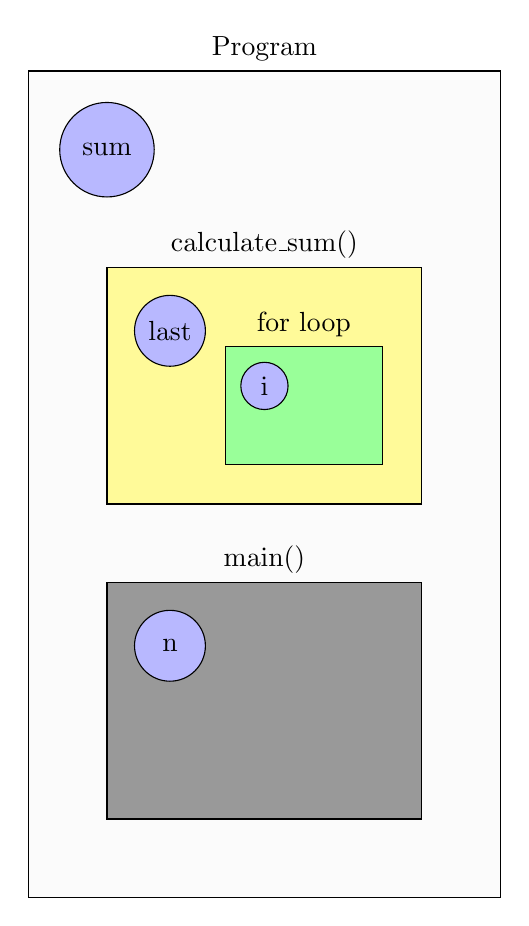
\begin{tikzpicture}\centering
		% program box
		\draw[fill=mygray] (-3,0) node [text=black,anchor=south,xshift=3cm] {Program} rectangle (3,-10.5) ;
		
		% calculate sum box
		\draw[fill=myyellow] (-2,-2.5) node [text=black,anchor=south,xshift=2cm] {calculate\_sum()} rectangle (2,-5.5) ;
		
		% for sub-box
		\draw[fill=mygreen] (-0.5,-3.5) node [text=black,anchor=south,xshift=1cm] {for loop} rectangle (1.5,-5) ;
		
		% main box
		\draw[fill=myblack]
		(-2,-6.5) node [text=black,anchor=south,xshift=2cm] {main()} rectangle (2,-9.5) ;
		
		\draw[fill=myblue] (-2,-1) circle (0.6) (-2,-1)  node [text=black] {sum}		% global variable sum
		(-1.2,-3.3) circle (0.45) (-1.2,-3.3)  node [text=black] {last}				% calculate_sum last
		(0,-4) circle (0.3) (0,-4)  node [text=black] {i} 							% for loop i
		(-1.2,-7.3) circle (0.45) (-1.2,-7.3)  node [text=black] {n} ;				% main n
	\end{tikzpicture}
\end{center}\bigbreak\bigbreak

If the above program were written using local variables (passing by value) instead, one could write:\\

\begin{lstlisting}
	#include <iostream>
	using namespace std;
	
	int calculate_sum(int last){
		int result = 0;		// local variable
		
		for(int i = 0; i <= last; i++) {
			result += i;
		}	
		
		return result;
	}
	
	int main(){
		int sum;		// local variable
		
		sum = calculate_sum(5);
		
		cout << sum;
	}
\end{lstlisting}\bigbreak


\subsubsection{Reference parameters}
\bigbreak

The parameters we've used so far are called \textbf{value parameters}. When a function is called, the \textbf{value} of the actual parameter \textbf{is copied} into the formal parameter. In that case, we say that parameters are \textbf{passed by value}.\\

When we passing by value, formal and actual parameters are \textbf{physically different} and only values can be passed. That is to say, both the formal and actual parameters have different locations in memory. Therefore, \textit{changes to the formal parameter in the function will not affect the actual parameter}. For example, \\

\begin{lstlisting}
	void foo(int last){
		last = 2;
	}
	
	int main(){
		int n = 5;
		
		foo(n);
		
		// n is still 5, it has not been changed by foo()
	}
\end{lstlisting}\bigbreak



An alternative solution is to pass parameters \textbf{by reference}. These are called \textbf{reference parameters}. In this case, the formal parameter (in the function header) \textit{is not a local variable} within the function.\\

The function will instead have access to the \textit{actual parameter} within the main. The function can use the value of the actual parameter from the main (a local variable to main) and change it directly. \\

To pass a parameter by reference in C++, we use the \& symbol. For example,\\


\begin{lstlisting}
	void foo(int &last){
		last = 2;
	}
	
	int main(){
		int n = 5;
		
		foo(n);
		
		// n is now 2, it has been changed by foo()
	}
\end{lstlisting}\bigbreak

Any change to last will affect n because of the use of the \& character. We would say that the variable last is a \textbf{pointer} for the variable n. There is \textit{no new variable physically} (in memory), last is simply another name for n.\\

When passing by value, a function can only calculate one value and return to the main. However, all parameters passed by reference can be changed by the function within the main. Therefore, \textit{if we want to return multiple values}, we can use a function of type void and pass parameters by reference if we need to calculate multiple values by a function.\\

We will now repeat the local and global variable (passing by value) example, now adjusted to pass by parameter.\\
\begin{lstlisting}
	#include <iostream>
	using namespace std;
	
	void calculate_sum(int &result, int last) {
		for(int i = 0; i <= last; i++) {
			result += i;
		}
	}
	
	int main(){
		int sum = 0;
		
		calculate_sum(sum, 5);
		
		cout << sum;
	}
\end{lstlisting}\bigbreak

Note that the parameter result is passed by reference, but the parameter last is passed by value.\\

Note also that we can not pass a constant by reference, since it has no location in memory.\\


\subsection{Arrays}
\bigbreak

An array is a \textbf{structure} for storing \textbf{multiple values} of the \textbf{same type}.\\

For example, suppose we are reading the numbers 5, 10, 3, 12, and 1.\\

We could find the largest of the values and print the result and it's index in the list (here, 12 fourth position). This is much more convenient for large data, when, for instance, reading each input in a different integer variable (a=5, b=10, etc.). \\

Instead, we could store all the values in one structure that is an array. The type of the array is int and the size is 5. All elemetns in the array are associateed with an incremental index that starts from zero.

\begin{center}
	\begin{table}[h]\centering
		\begin{tabular}{|c|c|c|c|c|c|}\hline
			index & 0 & 1 & 2 & 3 & 4 \\ \hline
			element & 5 & 10 & 3 & 12 & 1 \\ \hline
		\end{tabular}
	\end{table}
\end{center}

\subsubsection{Defining arrays}
\bigbreak

We can define an array of type int with size 34 as follows:

\begin{lstlisting}
	int marks[34];  // define but not initialized
\end{lstlisting}\bigbreak

Often it is useful to create a constant variable for the size of the array.

\begin{lstlisting}
	int SIZE = 34
	int marks[SIZE];  // define but not initialized
\end{lstlisting}\bigbreak

We can also initialize arrays.

\begin{lstlisting}
	int numbers[5] = {6, 3, -2, 0, 10};  // defined and initialized
\end{lstlisting}\bigbreak

There is no need to put the size of the array if we initialize it.

\begin{lstlisting}
	int numbers[] = {6, 3, -2, 0, 10};  // defined and initialized
\end{lstlisting}\bigbreak

If we give a size that is different from what is initialized. If the given size is greater than the size of the array passed to be initialized, it will fill the rest with zeros. Otherwise, if the given size is less than the size of the array passed to be initialized, it will give an error. 

\begin{lstlisting}
	int special[5] = {6, 3};  				// special = [6, 3, 0, 0, 0]
	int error[2] = {6, 3, -2, 0, 10};		// This results in a compile error
\end{lstlisting}\bigbreak

If we want an array of size 5 to be initialized with all 0s, we can do

\begin{lstlisting}
	int grades[5] = {};
\end{lstlisting}\bigbreak

You can also declare an array of other types.

\begin{lstlisting}
	string names[34]; 								// names = ["", "", ...]
	char vowels[] = {'a', 'e', 'i', 'o', 'u'};
\end{lstlisting}\bigbreak


\subsubsection{Accessing array elements}
\bigbreak

We can access arrays using square brackets as follows. We can read/write as with regular variables.

\begin{lstlisting}
	int A[5];
	
	A[3] = 25;					\\ set value at index 3 to 25
	A[4] = A[3] + 1;			\\ set value at index 4 to the value at index 3 plus one
\end{lstlisting}\bigbreak

If we want to print the contents of an array, we must iterate through each of the elements and print them individually.

\begin{lstlisting}
	for (int i=0;i<5;i++){
		cout << A[i] << endl;
	}
\end{lstlisting}\bigbreak

Since we have not initialized A[0], A[1], and A[2], they contain \textbf{garbage} (arbitrary, meaningless values).\\


The following is an example code to enter a sequence of grades using an array and calculate various properties of the set.\\

\begin{lstlisting}
	#include <iostream>
	using namespace std;
	
	int main(){
		
		int Grades[5] = {}; 	// initialized with zeros
		int grade;
		int size = 0;
		

		// Get grades
		for(int i=0;i<5;i++){
			
			cout << "Please enter a grade or -1 to quit: ";
			cin >> grade;
			
			if(grade == -1){
				break;		// exits for loop
			} else {
				Grades[i] = grade;
				size++;
			}
		}
		
		
		// Calculate average of grades
		int sum = 0;
		
		for(int i=0; i<size; i++) {
			sum = sum + Grades[i];
		}
		
		double average = sum/(double)size;
		
		cout << "Average is: " << average;
		
		
		/// Find the maximum and minimum grades
		
		int max = Grades[0];
		int min = Grades[0];
		
		for(int i=1; i<size; i++) {
			if(Grades[i] > max) {
				max = Grades[i];
			}
			if(Grades[i] < min) {
				min = Grades[i];
			}
		}
		
		cout << "Max is: " << Max << endl;
		cout << "Min is: " << Min << endl;
	
		return 0;
	}
\end{lstlisting}\bigbreak

\subsection{Implementation of Algorithms}

\subsubsection{The Sequential Search Algorithm\\ {\normalfont November 2nd, 2021}} \label{sequentialsearchalgorithm}
\bigbreak

Given a dataset of a given size $N$ and given a target, is the target in the dataset?\\

For example, if the dataset is the list [13, 4, 5, -20, 45, 112] with $N = 6$. Is the target 45 in the dataset? Yes. Is the target 130 in the dataset? No. \\

To solve for much larger values of N, we can search sequentially through the list until we reach the target (the target is in the list), or the end of the list (the target is not in the list).\\

Let us assume we have a list of size $N$ whose elements are $L_1$, $L_2$, ..., $L_N$ and a target element called Target.

\begin{algorithm}
	\caption{\\Sequential Search Algorithm}
	\begin{algorithmic}[1]
		\Get $L_1$, $L_2$, ..., $L_N$, $N$, Target
		\Set Found = No
		\Set $i$ = 1
		\While{Found = No AND $i$ <= $N$}
		\If{($L_i$ == Target)}
		\Set Found = Yes
		\Else
		\Set $i$ = $i$ + 1
		\EndIf
		\EndWhile
		\If{Found = Yes}
		\Print "Target in list."
		\Else
		\Print "Target not in list."
		\EndIf
		\Stop
	\end{algorithmic}
\end{algorithm}\bigbreak

We can implement the sequential search algorithm in C++ with the following code.

\begin{lstlisting}
	#include <iostream>
	using namespace std;
	
	int main(){
		
		// Declarations
		const int N = 10;
		int data[N];		// data is L in the algorithm
		int target;
		
		// Read data
		cout << "Please enter " << N << " elements: ";
		for (int i=0; i<N; i++)
			cin >> data[i];
		
		cout << "Please enter a target: ";
		cin >> target;
		
		// Search
		bool found = false;
		int index = 0;
		while(!found && index<N) {
			if (data[index] == target)
				found = true;
			else
				index++;
		}
		
		if(found)
			cout << "Target is in the list at index " << index << endl;
		else
			cout << "Target is not in the list" << endl;
		
		return 0;
	}
\end{lstlisting}\bigbreak


\subsubsection{The Selection Sort Algorithm} \label{selectionsort}
\bigbreak

Given a list of $n$ elements, we need to sort the list from smallest to largest.\\

For example, if the ($n = 5$) list = 5, 7, 2, 8, 3, then the sorted list should = 2, 3, 5, 7, 8.\\

Let's say we have the $n = 4$ list

\[
\renewcommand\arraystretch{1.5}
\begin{array}{|C|C|C|C!{\color{red}\vline}}\hline
	2 & 15 & 8 & 7 \\\hline
	\multicolumn{1}{c}{~} & \multicolumn{1}{c}{\color{red}\uparrow} & \multicolumn{1}{c}{~} & \multicolumn{1}{c}{~}
\end{array}
\]\bigbreak

We scan the list and find the largest (denoted by the red arrow). We also start with a marker (red line) equal to the length of the list. Then, we swap the element at that index with the last element and decrement the marker. Then, we repeat on all elements before the marker.

\[
\renewcommand\arraystretch{1.5}
\begin{array}{|C|C|C!{\color{red}\vline}C|}\hline
	2 & 7 & 8 & 15 \\\hline
	\multicolumn{1}{c}{~} & \multicolumn{1}{c}{~} & \multicolumn{1}{c}{\color{red}\uparrow} & \multicolumn{1}{c}{~}
\end{array}
\]\bigbreak

\[
\renewcommand\arraystretch{1.5}
\begin{array}{|C|C!{\color{red}\vline}C|C|}\hline
	2 & 7 & 8 & 15 \\\hline
	\multicolumn{1}{c}{~} & \multicolumn{1}{c}{\color{red}\uparrow} & \multicolumn{1}{c}{~} & \multicolumn{1}{c}{~}
\end{array}
\]\bigbreak

\[
\renewcommand\arraystretch{1.5}
\begin{array}{|C!{\color{red}\vline}C|C|C|}\hline
	2 & 7 & 8 & 15 \\\hline
	\multicolumn{1}{c}{\color{red}\uparrow} & \multicolumn{1}{c}{~} & \multicolumn{1}{c}{~} & \multicolumn{1}{c}{~}
\end{array}
\]\bigbreak

\[
\renewcommand\arraystretch{1.5}
\begin{array}{!{\color{red}\vline}C|C|C|C|}\hline
	2 & 7 & 8 & 15 \\\hline
\end{array}
\]\bigbreak\bigbreak

Now, the list is sorted. We can write the algorithm.\\

\begin{algorithm}
	\caption{\\Selection Sort}
	\begin{algorithmic}[1]
		\Get $n, L_1, ..., L_n$
		\Set Marker = $n$
		\While{(Marker > 1)}
		\Set largest = FindLargest($L_1, ..., L_{\mathrm{Marker}}$)
		\State Swap(largest, $L_{\mathrm{Marker}}$)
		\Set Marker = Marker - 1
		\EndWhile
		\Stop
	\end{algorithmic}
\end{algorithm}

We can implement the selection sort algorithm in C++ with the following code.

\begin{lstlisting}
	#include <iostream>
	using namespace std;
	
	int main(){
		
		// Declarations
		const int N = 10;
		int data[N];		// data is L in the algorithm
		
		// Read data
		cout << "Please enter " << N << " elements: ";
		for (int i=0; i<N; i++)
			cin >> data[i];
		
		// Sort
		for(int marker = N-1; marker>0; marker--){
			
			// find index with the largest value
			int largest = 0;
			for (int i=1; i<=marker;i++) {	
				if(data[i] > data[largest]) {
					largest = i;
				}
			}
		
			// swap L_largest and L_marker
			int temp = data[largest];
			data[largest] = data[marker];
			data[marker] = temp;
			
		}
		
		// Return list
		for (int i = 0; i<N; i++)
			cout << data[i] << " ";
		
		return 0;
	}
\end{lstlisting}\bigbreak



\subsubsection{The Binary Search Algorithm} \label{binarysearch}
\bigbreak

The objective of this algorithm is to search for an item in a list.\\

The \textit{sequential search} is one way to do this. Recall that it has a complexity of $\Theta(n)$. \textit{Can we make the search faster?}\\

The answer is \textbf{yes, but the list must be sorted}. If the list is sorted, then we can use the \textbf{binary search} (also called the \textit{half interval search}).\\

For example, we will use the following list with $n = 7$.

\[
\renewcommand\arraystretch{1.5}
\begin{array}{|C|C|C|C|C|C|C|}\hline
	5 & 16 & 25 & 32 & 38 & 57 & 58 \\\hline
	\multicolumn{1}{c}{\color{green}\uparrow} & \multicolumn{1}{c}{} & \multicolumn{1}{c}{} & \multicolumn{1}{c}{\color{blue}\uparrow} & \multicolumn{1}{c}{} & \multicolumn{1}{c}{} & \multicolumn{1}{c}{\color{red}\uparrow}
\end{array}
\]

And let our be target = 57.\\

We will define Start = 1 and End = 7 and we will also define Mid = $\frac{\mathrm{Start + End}}{2}=\frac{1 + 7}{2} = 4$. The value at the index Start is denoted by the green colored arrow, End by the red colored arrow, and Mid by the blue colored arrow. \\

We then get the value at mid and check if it is less than target. It is, therefore, we set start = mid + 1 = 5. And we recalculate mid =  $\frac{\mathrm{Start + End}}{2}=\frac{5 + 7}{2} = 6$. Our new list is


\[
\renewcommand\arraystretch{1.5}
\begin{array}{|C|C|C|C|C|C|C|}\hline
	5 & 16 & 25 & 32 & 38 & 57 & 58 \\\hline
	\multicolumn{1}{c}{} & \multicolumn{1}{c}{} & \multicolumn{1}{c}{} & \multicolumn{1}{c}{} & \multicolumn{1}{c}{\color{green}\uparrow} & \multicolumn{1}{c}{\color{blue}\uparrow} & \multicolumn{1}{c}{\color{red}\uparrow}
\end{array}
\]

Now, we get the value at mid which is 57. We check if it equals our target and it does, therefore, we say that our target is found (and at the index mid). We stop the algorithm there. \\

For this particular setup, it took 2 iterations. This is much faster than the 6 steps that it would have taken to do with sequential search.\\

Does this mean that the binary search is better than sequential search? Well, for finding a target it is. However, there is some time that is taken when initially sorting the list in the first place. If fast storage of data is required, perhaps the binary search is not the best option.\\

We will build now the algorithm.

\begin{algorithm}
	\caption{\\Binary Search}
	\begin{algorithmic}[1]
		\Get $n, L_1, ..., L_n$
		\Get Target
		\Set Found = No
		\Set Start, End = 1, N
		\While{(Found = No AND Start $\ne$ End)}
		\Set Mid = $\frac{\mathrm{Start + End}}{2}$
		\If{($L_{\mathrm{Mid}}$ = Target)}
		\Set Found = Yes
		\Else
		\If{(Target < $L_{\mathrm{Mid}}$)}
		\Set End = Mid - 1
		\Else
		\Set Start = Mid + 1
		\EndIf
		\EndIf
		\EndWhile
		\If{(Found = Yes)}
		\Print "Target found"
		\Else
		\Print "Target not found"
		\EndIf
		\Stop
	\end{algorithmic}
\end{algorithm}

We can implement the binary search algorithm in C++ with the following code.

\begin{lstlisting}
	#include <iostream>
	using namespace std;
	
	int main(){
		
		// Declarations
		const int N = 10;
		int data[N];		// data is L in the algorithm
		int target;
		
		// Read data
		cout << "Please enter " << N << " sorted elements: ";
		for (int i=0; i<N; i++)
		cin >> data[i];
		
		cout << "Please enter a target: ";
		cin >> target;
		
		// Search
		bool found = false;
		int start = 0;
		int last = N - 1;       // last is End in the algorithm
		int mid;
		
		while (!found && start < last){
			mid = (start + last)/2;
			if (data[mid] == target)
				found = true;
			else
				if(target < data[mid])
					last = mid - 1;
				else
					start = mid + 1;
		}
		
		if(found)
			cout << "Target is in the list at index " << mid << endl;
		else
			cout << "Target is not in the list" << endl;
		
		return 0;
	}

\end{lstlisting}\bigbreak


\subsection{Arrays and Functions\\ {\normalfont November 10th, 2021}}
\bigbreak

Sometimes it is useful to use arrays in functions.

\begin{itemize}
	\item An array can be passed as a parameter
	\item Arrays are passed by reference (their content can be changed by function)
	\item Formal parameter: no \& (reserved for scalar values), empty [] instead
	\item Actual parameter: array name without []
	\item Cannot return an array (only a single value)
\end{itemize}\bigbreak

An example of using arrays in a function is

\begin{lstlisting}
	int sum(int values[], int size) {
		int total = 0;
		for (int i=0; i<size; i++)
			total += values[i]
		return total
	}
\end{lstlisting}\bigbreak

A \textbf{bad example} (one that will give an error) is the following, if you try to return an array:

\begin{lstlisting}
	int[] getinfo(){
		cout << "How many: ";
		int size;
		cin >> size;
		int data[size];
		for (int i=0; i< size; i++)
			cin >> data[i];
		return data
	}
\end{lstlisting}\bigbreak

Instead, you must pass by parameter:

\begin{lstlisting} 
	void getinfo(int data[], int &size) {
		cout << "How many: ";
		cin >> size;
		for (int i=0; i<size; i++)
			cin >> data[i];
	}
\end{lstlisting}\bigbreak

The following code is an example of various functions that involve arrays in the parameters or return.

\begin{lstlisting}
	#include <iostream>
	using namespace std;
	
	int readarray(int data[]){
		int len;
		cout << "What is the length of the array (less than 100): ";
		cin >> len;
		
		for(int i=0; i< len; i++)
			cin >> data[i];
		
		return len;
	}
	
	void multiplyarray(int data[], int len, int factor){
		for(int i=0; i< len; i++)
			data[i] = data[i] * 2;
	}
	
	void printarray(int data[], int len){
		for(int i=0; i< len; i++)
			cout << data[i] << endl;
	}
	
	int main(){
		const int MAXSIZE = 100;
		
		int data[MAXSIZE];
		int len;
		
		len = readarray(data);
		multiplyarray(data, len, 2);
		printarray(data, len);
	}
\end{lstlisting}\bigbreak

\subsubsection{2D Arrays}
\bigbreak

We often need to use arrays within arrays. These are called \textbf{2D arrays}. An example of a 1D array of size 7 is\bigbreak

\[
\renewcommand\arraystretch{1.5}
\begin{array}{|C|C|C|C|C|C|C|}\hline
	5 & 16 & 25 & 32 & 38 & 57 & 58 \\\hline
\end{array}
\]
\bigbreak
Whereas a 2D array with 3 rows and 7 columns could be
\bigbreak
\[
\renewcommand\arraystretch{1.5}
\begin{array}{|C|C|C|C|C|C|C|}\hline
	70 & 5 & 53 & 62 & 3 & 91 & 13 \\\hline
	12 & 7 & 82 & 7 & 9 & 19 & 40 \\\hline
	2 & 98 & 21 & 4 & 84 & 75 & 25 \\\hline
\end{array}
\]
\bigbreak

In C++ code, we can declare a 2D array with 

\begin{lstlisting}
	const int maxrows = 4;
	const int maxcols = 3;
	
	int counts[maxrows][maxcols];  		// declare but not initialize
\end{lstlisting}\bigbreak

We can also initialize 2D arrays as follows:

\begin{lstlisting}
	int grades[3][2] = {{85,69},{77,98},{87,83}}; 	// declare and initialize
\end{lstlisting}\bigbreak

Similar to the 1D array, when initializing, you can leave out the first size.

\begin{lstlisting}
	int marks[][2] = {{85,69},{77,98},{87,83}};	
\end{lstlisting}\bigbreak

We will do an example problem where we need to store and count the number of medals (gold, silver, and bronze) won by 4 countries. For instance, we could have the case where the countries' medal count can be represented in the table

\begin{table}[ht!]\hskip3.9cm
	\renewcommand\arraystretch{2}
	\begin{tabular}{r|c|c|c|}
		\multicolumn{1}{c}{} & \multicolumn{1}{c}{~gold~} & \multicolumn{1}{c}{silver} & \multicolumn{1}{c}{bronze}  \\\cline{2-4}
		country 1 & 5 & 2 & 6 \\\cline{2-4}
		country 2 & 3 & 9 & 8 \\\cline{2-4}
		country 3 & 2 & 3 & 1 \\\cline{2-4}
		country 4 & 2 & 0 & 7 \\\cline{2-4}
	\end{tabular}
	\bigbreak
\end{table}

The full code is

\begin{lstlisting}
	#include <iostream>
	using namespace std;
	
	string country(int label) {
		switch(label) {
			case 0: return "Canada";
			case 1: return "USA";
			case 2: return "China";
			case 3: return "France";
			default: return "";
		}
	}

	string medal(int label) {
		switch(label) {
			case 0: return "Gold";
			case 1: return "Silver";
			case 2: return "Bronze";
			default: return "";
		}
	}

	
	int main() {
		// declare values and constants
		const int COUNTRIES = 4;
		const int MEDALS = 3;
		int counts[COUNTRIES][MEDALS];
		
		// fill array and calculate the sums of rows
		for(int i=0; i<COUNTRIES; i++) {
			cout << "Enter the medals counts for " << country(i) << ": ";
			for(int j=0;j<MEDALS;j++)
				cin >> counts[i][j];
		}
		cout << endl;
		
		// calculate the sums of rows
		for(int i=0; i< COUNTRIES; i++){	
			int sum = 0;
			for(int j=0; j<MEDALS; j++)
				sum += counts[i][j];
			cout << "The total number of medals won by " << country(i) << " is " << sum << endl;
		}
		cout << endl;
		
		// calculate the sums of columns
		for(int j=0; j< MEDALS; j++){
			int sum = 0;
			for(int i=0; i<COUNTRIES; i++)
				sum += counts[i][j];
			cout << "The total number of " << medal(j) << " medals is " << sum << endl;
		}
		cout << endl;
		
		/// display array
		for(int i=0; i<COUNTRIES;i++){
			for(int j=0;j<MEDALS;j++)
				cout << counts[i][j] << " ";
			cout << endl;			
		}
		cout << endl;
	}
\end{lstlisting}\bigbreak

You could also construct a function fillarray() which fills the array from a function instead of from the main. However, the number of rows and number of columns constants must be made globally so that the fillarray can access it.

\begin{lstlisting}
	const int COUNTRIES = 4;
	const int MEDALS = 3;
	
	void fillarray(int counts[][MEDALS]){
		for(int i=0; i<COUNTRIES; i++) {
			cout << "Enter the medals counts for " << country(i) << ": ";
			for(int j=0;j<MEDALS;j++)
				cin >> counts[i][j];
		}
		cout << endl;
	}

	int main() {
		int counts[COUNTRIES][MEDALS];
		
		fillarray(counts);
		
		...
	}
\end{lstlisting}\bigbreak


\subsection{Vectors}
\bigbreak

Arrays are not the only data structure that can store multiple values, we can also use \textbf{vectors}.

\begin{itemize}
	\item A vector collects a sequence (1D, 2D, etc.) of same type values just like an array does
	\item Unlike arrays, the size of a vector can change
	\item A vector is a higher abstraction of array: Array with a lot of useful built-in functions.
\end{itemize}\bigbreak

To use vectors in C++, we need to include the package.

\begin{lstlisting}
	#include <vector>
\end{lstlisting}\bigbreak

To declare a vector (let's say one that contains doubles), we can write

\begin{lstlisting}
	vector <double> marks;		// initial size is 0
\end{lstlisting}\bigbreak

We can declare an initial size with following parentheses

\begin{lstlisting}
	vector <double Marks(10);		// initial size is 10
\end{lstlisting}\bigbreak

If we want to get the \textbf{current size} of a vector, we can use

\begin{lstlisting}
	int size =  Marks.size();
\end{lstlisting}\bigbreak

To fill a vector with inputted values, we can use

\begin{lstlisting}
	for(int=0; i < Marks.size(); i++)
		cin >> Marks[i];
\end{lstlisting}\bigbreak

The vector has a few more conveniences:

\begin{itemize}
	\item Vectors can be used in functions like any other variable
	\item They can be passed by reference (with the \&) or by value
	\item They can be returned by a function
\end{itemize}\bigbreak

To see the complete list of builtin functions for the vectors, visit the reference documentation at \url{https://www.cplusplus.com/reference/vector/vector/}.\\

As an example, let us make a vector that contains students marks. First, we can employ the following strategy if the size is known.

\begin{lstlisting}
	// declare
	vector <double> marks(10);
	
	// fill
	for(int=0; i < marks.size(); i++)
		cin >> marks[i];
	
	// display
	for(int=0; i < marks.size(); i++)
		cout << marks[i] << endl;
\end{lstlisting}\bigbreak

However, if the size is unknown, we can instead do the following to fill the vector.

\begin{lstlisting}
	// The user enters values and stops when q is entered
	double grade;
	while (cin >> grade) {	// 1. A value is read  2. returns true/false based on type of value
		marks.push_back(grade);		// increases the size by one and put grade in that location 
	}
	cin.clear();
	cin.ignore();
\end{lstlisting}\bigbreak

This shows you how to increase the size of a vector, but how do you \textit{decrease} the size of a vector? We can pop the last value off of the vector and decrement the size by one. This is done with

\begin{lstlisting}
	marks.pop_back();	// removes last cell of the vector
\end{lstlisting}\bigbreak

To get the first and last elements of a vector, we can use the following methods

\begin{lstlisting}
	// First grade
	cout << marks[0] << endl;
	cout << marks.front() << endl;
	
	// Last grade
	cout << marks[marks.size() - 1] << endl;
	cout << marks.back() << endl;
\end{lstlisting}\bigbreak 


To calculate the average grade,

\begin{lstlisting}
	double total = 0;
	double average;
	for (int i=0; i < marks.size; i++)
		total += marks[i];
	
	if (marks.size() != 0)
		average = total / marks.size();
	else {
		cout << "No data. Program will stop";
		return -1;
	}

	cout << "Average is: " << average << endl;
\end{lstlisting}\bigbreak

To find and remove the smallest grade,

\begin{lstlisting}
	// find position of smallest
	int smallpos = 0;
	for(int i=0; i < marks.size(); i++) {
		if (marks[i] < marks[smallpos]) {
			smallpos = i;
		}
	}
	
	// copy back of vector to smallpos and remove duplicated back value
	marks[smallpos] = marks.back();
	marks.pop_back();
\end{lstlisting}\bigbreak


We can make the reading of a vector to be a function using the following

\begin{lstlisting}
	vector<double> vect_read() {
		vector <double> v;
		
		double element;
		while(cin >> element)
			v.push_back(element);
		cin.clear();
		cin.ignore();
		
		return v;
	}
\end{lstlisting}\bigbreak

We can also make the finding of the average of the elements of a vector using

\begin{lstlisting}
	vector<double> vect_avg(vector<double> v) {
		double total = 0;
		
		for(int i=0; i< v.size();i++){
			total += v[i];
		}
	
		if (v.size()!=0)
			return total / v.size();
		
		return -1;  // Error, no data
	}
\end{lstlisting}\bigbreak


Finally, we can finding the smallest element of a vector with yet another function if we want:

\begin{lstlisting}
	int vect_minpos(vector<double> v) {
		int index = 0;
		for (int i=0; i<v.size();i++) {
			if (v[i] < v[index])
				index = i;
		}
		return index;
	}
\end{lstlisting}\bigbreak

We can make a remove function if we would like also, to remove the element of a particular position

\begin{lstlisting}
	void vect_remove(vector<double> &results, int index) {
		results[index] = results.back();
		results.pop_back();
	}
\end{lstlisting}\bigbreak


To append a vector (source) to another one (destination), we can use the function

\begin{lstlisting}
	void append(vector<int> src, vector<int> &dest) {
		for (int i=0; i<src.size(); i++) {
			dest.push_back(src[i]);
		}
	}
\end{lstlisting}\bigbreak

We can print a vector with something like

\begin{lstlisting}
	void print(vector<int> v) {
		for (int i=0; i<v; i++) {
			cout << v[i] << " ";
		}
		cout << endl;
	}
\end{lstlisting}\bigbreak

Something to note about arrays is that you cannot simply assign one to another, you must assign each element to another. Namely, 

\begin{lstlisting}
	int A[2] = {1, 6};
	int B[2];
	
	B = A; // Gives Error
	
	for (int i=0; i<2; i++)	// Must iterate over all elements instead
		B[i] = A[i];
\end{lstlisting}\bigbreak

Whereas for vectors, you can directly assign one to the another without error.

\begin{lstlisting}
	vector <int> A(2);
	A[0] = 1;
	A[1] = 6;
	vector <int> B;
	
	B = A; 	// This works now
	
	for (int i=0; i<A.size(); i++)	// This still also works
		B.push_back(A[i]);
\end{lstlisting}\bigbreak


\subsection{Pointers}
\bigbreak

\subsubsection{The reference operator: \&}
\bigbreak

A variable is stored in the memory and a variable is associated with a \textit{memory address} which points to a particular cell in memory.\\

If we have a variable, we can find the address of the number using the ampersand sign (\&). For instance,

\begin{lstlisting}
	int number = 25;
	
	cout << "number = " << number << endl;
	cout << "Address of number = " << &number << endl; 
\end{lstlisting}\bigbreak

This will give us a result in hexadecimal such as 0x6dfefc.\\

If we also pass it through a function \textbf{by value} as follows 

\begin{lstlisting}
	int number = 25;
	
	cout << "number = " << number << endl;
	cout << "Address of number = " << &number << endl << endl; 
	
	display(number);
\end{lstlisting}\bigbreak

where display is defined as

\begin{lstlisting}
	void display(int number) {
		cout << "In a function:" << endl;
		cout << "number = " << number << endl;
		cout << "Address of number = " << &number << endl; 
	}
\end{lstlisting}\bigbreak

we will get a \textit{different memory address}, but the same value for the variable (e.g. 0x6dfefc and 0x6dfee0). We can clearly see the locality of the variables this way.\\

If instead we pass number \textbf{by reference} to display with 

\begin{lstlisting}
	void display(int &number) {
		cout << "In a function:" << endl;
		cout << "number = " << number << endl;
		cout << "Address of number = " << &number << endl; 
	}
\end{lstlisting}\bigbreak

Then we can see that they both have the \textit{same address} (e.g. 0x6dfefc and 0x6dfefc).\\

The ampersand sign (\&) is called the \textbf{reference operator} and it allows access to values' addresses.\\


\subsubsection{Definition of Pointers}
\bigbreak

\begin{itemize}
	\item A variable contains a value: int number = 25;
	\item The address of a variable is acessed by \&: Address of number is \&number
	\item A pointer is a special type of variable that contains an address.
	\item For example: \begin{lstlisting}
		int *p;
	\end{lstlisting}
	\item p is a pointer to a variable that contains an int
	\item p will contain the address of a variable of type int.
	\item * is called the \textbf{dereference operator} (*p: value pointed by p) 
\end{itemize}\bigbreak


We can define a pointer called p using

\begin{lstlisting}
	int *p;
\end{lstlisting}\bigbreak

If we want to initialize the pointer, we need to define another variable (say number) and then define it to be the address of that variable.

\begin{lstlisting}
	int number = 25;	// initialize another variable
	int *p;				 // declare pointer
	p = &number;		 // assign pointer the address of another variable
\end{lstlisting}\bigbreak


If we write

\begin{lstlisting}
	*p = 35;
\end{lstlisting}\bigbreak

We take the number at the address pointed to by p to be 35. Thus, number becomes equal to 35.\\

If we declare new\_number, if we want to set p to point to new\_number instead of number, we must not use the *

\begin{lstlisting}
	int new_number;
	p = &new_number;
\end{lstlisting}\bigbreak

Now p points to new\_number and not to number anymore. So if we assign the value at p to be 40 with 

\begin{lstlisting}
	*p = 40;
\end{lstlisting}\bigbreak

then new\_number becomes 40, but number is still 35.\\

We will now do a few examples of this.\\

\textbf{Example 1:}

\begin{lstlisting}
	// Declaration and Assignment of Pointers
	int number = 25;
	
	cout << "number = " << number << endl;				// 25
	cout << "address number = " << &number << endl;		// 0x6dfef8
	
	int *p;
	p = &number
	
	cout << "p = " << p << endl; 		// 0x6dfef8
	cout << "*p = " << *p << endl;		// 25
	
	double new_number = 56.0;
	p = &new_number;		// Error, p must point to an int, new_number must instead be an int
\end{lstlisting}\bigbreak

\textbf{Example 2:}

\begin{lstlisting}
	// Manipulation with the pointers
	
	int first = 5;
	int sec = 15;
	
	int *p1, *p2;
	p1 = &first;
	p2 = &sec;
	// first = 5, second = 15, *p1 = 5, *p2 = 15
	
	*p1 = 10;
	// first = 10, second = 15, *p1 = 10, *p2 = 15
	
	*p2 = *p1;
	// first = 10, second = 10, *p1 = 10, *p2 = 10
	
	p1 = p2;
	// first = 10, second = 10, *p1 = 10, *p2 = 10
	// p2 now points to first
	
	*p1 = 20;
	// first = 10, second = 20, *p1 = 20, *p2 = 20
	
	cout << first << " " << sec << " " << *p1 << " " << *p2;
\end{lstlisting}\bigbreak

\textbf{Example 3:}

\begin{lstlisting}
	// Pointers initialization errors
	
	int *p1;
	*p1 = 25; 		// fatal error
	// This is because p1 does not point anywhere, and you cannot assign 25 to nowhere
	
	// Must do the following instead
	int number; 
	int *p1 = &number;
	int *p1 = 25;
\end{lstlisting}\bigbreak







\end{document}
